% Name: Complete graph
% Description: The complete graph K5: five vertices on a regular pentagon, with an edge between every pair, ten in all.
% Tags: complete graph, K5, graph theory

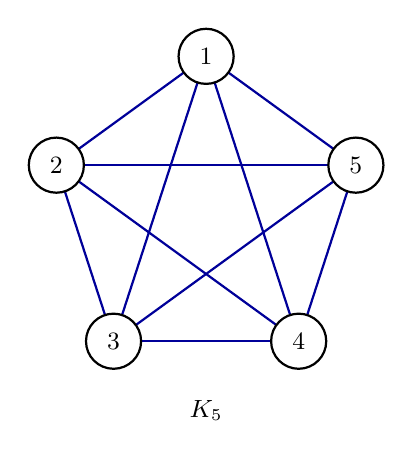
\begin{tikzpicture}[vertex/.style={circle, draw, thick, fill=white, minimum size=7mm, font=\small}]
  % Vertex i sits at angle 90 + 72i degrees on a circle of radius 2.
  \foreach \i in {1,...,5}
    \coordinate (v\i) at ({90+72*(\i-1)}:2);
  \foreach \i [evaluate=\i as \k using {int(\i+1)}] in {1,...,4}
    \foreach \j in {\k,...,5}
      \draw[thick, blue!60!black] (v\i) -- (v\j);
  \foreach \i in {1,...,5}
    \node[vertex] at (v\i) {$\i$};
  \node[font=\small] at (0,-2.5) {$K_5$};
\end{tikzpicture}
